%% Do not edit unless you really know what you are doing.
\documentclass[11pt]{article}
\usepackage{amsmath}
\usepackage{amssymb}
\usepackage{fontspec}
\setmainfont[Ligatures=TeX]{Calibri}
\usepackage{geometry}
\geometry{verbose,tmargin=2.54cm,bmargin=2.54cm,lmargin=3.5cm,rmargin=2.54cm}
\setcounter{secnumdepth}{0}
\setcounter{tocdepth}{3}
\usepackage{graphicx}
\usepackage{setspace}
\onehalfspacing
\usepackage[unicode=true,
 bookmarks=false,
 breaklinks=true,pdfborder={0 0 0},pdfborderstyle={},backref=section,colorlinks=false]
 {hyperref}

\makeatletter
\@ifundefined{date}{}{\date{}}
%%%%%%%%%%%%%%%%%%%%%%%%%%%%%% User specified LaTeX commands.
\PassOptionsToPackage{unicode=true}{hyperref} % options for packages loaded elsewhere
\PassOptionsToPackage{hyphens}{url}
%
\usepackage{ifxetex}
\usepackage{ifluatex}\usepackage{fixltx2e}% provides \textsubscript
\ifnum 0\ifxetex 1\fi\ifluatex 1\fi=0 % if pdftex
  \usepackage{textcomp}% provides euro and other symbols
\else % if luatex or xelatex
  \usepackage{unicode-math}
\defaultfontfeatures{Ligatures=TeX,Scale=MatchLowercase}
\fi
% use upquote if available, for straight quotes in verbatim environments
\IfFileExists{upquote.sty}{\usepackage{upquote}}{}
% use microtype if available
\IfFileExists{microtype.sty}{%
\usepackage[]{microtype}
\UseMicrotypeSet[protrusion]{basicmath} % disable protrusion for tt fonts
}{}
\IfFileExists{parskip.sty}{%
\usepackage{parskip}
}{% else
\setlength{\parindent}{0pt}
\setlength{\parskip}{6pt plus 2pt minus 1pt}
}

\urlstyle{same}  % don't use monospace font for urls
\setlength{\emergencystretch}{3em}  % prevent overfull lines
\providecommand{\tightlist}{%
  \setlength{\itemsep}{0pt}\setlength{\parskip}{0pt}}

% Redefines (sub)paragraphs to behave more like sections
\ifx\paragraph\undefined\else
\let\oldparagraph\paragraph
\renewcommand{\paragraph}[1]{\oldparagraph{#1}\mbox{}}
\fi
\ifx\subparagraph\undefined\else
\let\oldsubparagraph\subparagraph
\renewcommand{\subparagraph}[1]{\oldsubparagraph{#1}\mbox{}}
\fi

% set default figure placement to htbp

\def\fps@figure{htbp}
\usepackage{fontspec}
\setmainfont{Calibri}
\usepackage[utf8]{inputenc}

\makeatother

\begin{document}

\title{\textsc{Close-reading of Linked Data: a practical case study on the quality of online authority files}}

\author{Ettore Rizza, Anne Chardonnens, Seth van Hooland}
\maketitle

\section{Introduction}

More and more cultural institutions use Linked Data principles\footnote{Described in \textsc{T. Berners-Lee}, ``Design issues: Linked
data (2006)'', 2011, URL: \href{https://www.w3.org/DesignIssues/LinkedData.html}{https://www.w3.org/DesignIssues/LinkedData.html}
(accessed 14 September 2018). Namely : 1° Use~URIs~to name (identify)
things; 2° Use~HTTP~URIs so that these things can be looked up;
3° Provide useful information about what a name identifies when it's
looked up, using open standards such as~RDF,~SPARQL, etc; 4° Refer
to other things using their~HTTP~URI-based names when publishing
data on the Web.} to share and connect their collection metadata. In the archival field,
initiatives emerge to exploit data contained in archival descriptions
and adapt encoding standards to the semantic web\footnote{\textsc{K. F. Gracy}, ``Archival description and linked
data: a preliminary study of opportunities and implementation challenges'',
\emph{Archival Science}, 15(3), 2015, pp. 239–294.}. In this context, online authority files can be used to enrich metadata.
However, relying on a decentralized network of knowledge bases such
as Wikidata\footnote{\textsc{D. Vrandečić, M. Krötzsch}, ``Wikidata: a free collaborative
knowledge base'', \emph{Communications of the ACM}, 57(10), 2014,
pp. 78–85.}, DBpedia\footnote{\textsc{J. Lehmann, R. Isele, M. Jakob, A. Jentzsch, D. Kontokostas,
P. N. Mendes,\ldots{} others}, ``DBpedia–a large-scale, multilingual
knowledge base extracted from Wikipedia'', \emph{Semantic Web}, 6(2),
2015, pp. 167–195.} or even Viaf\footnote{\textsc{M. F. Loesch}, ``VIAF (The Virtual International
Authority File) – http://viaf.org'', \emph{Technical Services Quarterly},
28(2), 2011, pp. 255–256, \href{https://doi.org/10.1080/07317131.2011.546304}{https://doi.org/10.1080/07317131.2011.546304}} has its own difficulties. This paper aims to offer a critical view
of these linked authority files by adopting a \emph{close-reading}
approach. Through a practical case study, we intend to identify and
illustrate the possibilities and limits of RDF\footnote{Resource Description Framework. \textsc{D. Brickley, R. V. Guha, B.
McBride}, ``RDF vocabulary description language 1.0: RDF Schema.
W3C Recommendation'', 2004, URL:\href{http://www.W3.Org/Tr/2004/Rec-Rdf-Schema-20040210}{http://www.W3.Org/Tr/2004/Rec-Rdf-Schema-20040210}. } triples compared to institutions' less structured metadata.~

Our paper is an invitation to travel in an unexpected way: diving
through the Linked Open Data cloud\footnote{The LOD Cloud Graph, maintained since 2007, is an attempt to map the
Linked Open Data ecosystem. The last version (28 August 2018) contains
1224 linked datasets: \href{https://lod-cloud.net/}{https://lod-cloud.net/}
(accessed 14 September 2018).} by a ``thought experiment''. Let's suppose that we have a smart
robot able to jump from one dataset of RDF triples to another, for
example using SPARQL endpoints, and let's call it Alex. Alex is a
kind of computerized archivist. We will ask it to use the Linked Data
to get information about Henry Carton de Wiart (1869–1951), a famous
Belgian personality from the early 20th century. Part of a large noble
Walloon family, Carton de Wiart has been minister several times, Prime
Minister, president of many councils and organizations, and a lawyer
and a writer as well. The Belgian city Liège owes one of its nicknames
to one of his books, \emph{La Cité ardente}\footnote{\textsc{H. Carton de Wiart}, \emph{La Cité ardente, avec
une préface de M. Henry Bordeaux}, Paris, 1904. }. Moreover, he has been honored by several awards and was in contact
with many well-known personalities, from the French poet Verlaine
to the President of America Woodrow Wilson. His life contains therefore
enough facets to act as a case study to compare how Linked Open Data
can reconstruct a biography compared to more traditional information
sources.

Most of the studies about Linked Open Data quality adopt ``big data''
approaches based on methods such as data mining or network analysis.
They tend to analyze the data quality of datasets only through the
prism of quantitative and comparative analysis\footnote{\textsc{A. Zaveri, A. Rula, A. Maurino, R. Pietrobon, J. Lehmann,
S. Auer}, ``Quality assessment for linked data: A survey'', in
\emph{The Semantic Web}, 7(1), 2012, pp. 63–93.}. In this paper, we opt for a close-reading approach focusing on a
single individuality, in order to analyze how the triple structure
deals with historical/biographical data compared with traditional
authority files.

\section{Continuum}

This paper aims to reflect on the continuum of different documentation
practices and methods, from the traditional paper-based narrative
to very structured data published as RDF triples in knowledge graphs\footnote{This term, coined and popularized by Google in 2012, refers to knowledge
bases structured as RDF graphs.}. At one end are unstructured data, like the national biography of
Henry Carton de Wiart, an eight pages well-written text digitized
and published online in a PDF version\footnote{\textsc{Académie royale des Sciences, des Lettres et des Beaux-Arts
de Belgique}, \emph{Biographie Nationale}, Tome 44, Dernier Supplément,
tome XVI, Fasc. 1, Artoisenet-Eracle, 1985, Bruxelles, Retrieved from
\href{http://www.academieroyale.be/Academie/documents/FichierPDFBiographieNationaleTome2102.pdf }{http://www.academieroyale.be/Academie/documents/FichierPDFBiographieNationaleTome2102.pdf }.}. At the other end stand the most structured data, which corresponds
to Linked Data, such as the Wikidata resource for Henry Carton de
Wiart\footnote{\href{https://wikidata.org/wiki/Q14990}{https://wikidata.org/wiki/Q14990}
(accessed 14 September 2018).}, its Viaf authority file\footnote{\href{https://viaf.org/viaf/24623115}{https://viaf.org/viaf/24623115}(accessed
14 September 2018).} or its French DBpedia page\footnote{\href{http://fr.dbpedia.org/page/Henry_Carton_de_Wiart}{http://fr.dbpedia.org/page/Henry\_Carton\_de\_Wiart}(accessed
14 September 2018).}. In between are established more isolated structured data like RDF
triples from archives or libraries repositories\footnote{e.g. Data.bnf.fr: \href{http://data.bnf.fr/12062835/henry_carton_de_wiart/}{http://data.bnf.fr/12062835/henry\_carton\_de\_wiart/}
(accessed 14 September 2018).}, archival descriptions in XML\footnote{e.g. the EAC-CPF file from the State Archives of Belgium: \href{https://search.arch.be/eac/xml/eac-BE-A0500_007556_FRE.xml}{https://search.arch.be/eac/xml/eac-BE-A0500\_007556\_FRE.xml}
(accessed 14 September 2018).} or Wikipedia pages\footnote{e.g. the English version: \href{https://en.wikipedia.org/wiki/Henry_Carton_de_Wiart}{https://en.wikipedia.org/wiki/Henry\_Carton\_de\_Wiart}
(accessed 14 September 2018).}.

While the most structured resources display facts (such as a birth
date or death date) very clearly, in a machine-readable format, we
can wonder if they provide as many details as a more classical format
type, such as the national biography. Do they mention his origins
from Hainaut, his correspondence with an apostolic vicar living in
Brazzaville, or that day in August 1914 when the Belgian king asked
him to lead an extraordinary mission to the United States? These questions
can be mapped to the central premise of Lev Manovich's book \emph{The
Language of New Media}, which stresses the tension between traditional
narratives and databases\footnote{\textsc{L. Manovich, R. F. Malina, S. Cubitt},\emph{ The
Language of new media}, Cambridge, 2001.}. Through this case study, we aim to extend this thinking and confront
various forms of structured sources and to observe to what extent
they are consistent and complementary.

\section{Diving into the LOD cloud}

Alex-the-robot, the main fictional character of our case study, can
be seen as a cousin of the modern ``robot journalists'', these systems
able to write short texts—for example weather or financial reports—using
structured information\footnote{\textsc{L. Dierickx}, ``News bot for the newsroom: how building
data quality indicators can support journalistic projects relying
on real-time open data'', in \emph{Global Investigative Journalism
Conference 2017} Academic Track, Investigative Journalism Education
Consortium, 2017.}.

Alex, for its part, would write biographical texts based on information
extracted from the Linked Open Data cloud. It will proceed like a
historian who collects pieces of information from various sources,
to gradually be able to describe a personality. But instead of reading
archives or books, Alex would perform queries on the web and then
interpret the results, at least if these results are in a machine-readable
format such as XML, JSON, any RDF serialization and so on. Even if
it does not understand natural language, it is able to write basic
sentences, for example that someone was born that year, in that location,
and practiced this or that activity.

\begin{singlespace}
As a reminder, the principles of Linked Data advocate to use URIs
(Uniform Resource Identifiers) as names for things and to use standards
such as RDF. For example, the sentence ``the artwork \emph{Puppy}
held by the Guggenheim Museum was made by Jeff Koons'' can be expressed
in RDF as follows (using the N-triples notation)\footnote{Example borrowed from \textsc{S. Van Hooland, R. Verborgh},
\emph{Linked Data for Libraries, Archives and Museums: How to clean,
link and publish your metadata}, London, 2014.}: 
\end{singlespace}
\begin{singlespace}
\begin{center}
\textsf{<\href{http://www.guggenheim.org/new-york/collections/collection-online/artwork/48}{http://www.guggenheim.org/new-york/collections/collection-online/artwork/48}>}
\par\end{center}

\begin{center}
\textsf{<\href{http://purl.org/dc/terms/creator}{http://purl.org/dc/terms/creator}>}
\par\end{center}

\begin{center}
\textsf{<\href{http://viaf.org/viaf/5035739}{http://viaf.org/viaf/5035739}>}.
\par\end{center}
\end{singlespace}

As we said, Alex's first mission in this experiment is to collect
as many triples as possible about Henry Carton de Wiart. Its starting
point will be for example DBpedia, often considered as the central
point of the Linked Open Data cloud, since many datasets of the LOD
cloud are linked to it\footnote{\textsc{S. Auer, C. Bizer, G. Kobilarov, J. Lehmann, R. Cyganiak,
Z. Ives}, ``Dbpedia: A nucleus for a web of open data'', In \emph{The
Semantic Web}, 2007, pp. 722–735.}. Thus, we will ask Alex to go to the Carton de Wiart's English DBpedia
page\footnote{\href{http://dbpedia.org/page/Henri_Carton_de_Wiart}{http://dbpedia.org/page/Henri\_Carton\_de\_Wiart}
(accessed 14 September 2018).}, to collect RDF data from this page and then to follow all the links
to external databases using, for instance, the \textsf{owl:sameAs}\footnote{\href{https://www.w3.org/TR/owl-ref/\#sameAs-def}{https://www.w3.org/TR/owl-ref/\#sameAs-def}
(accessed 14 September 2018).} relations.

Figure~1 shows all the links between the knowledge bases used in
this experiment. As aforementioned, the entry point is DBpedia. All
the paths explored by Alex are visible. From DBpedia, Alex goes to
various versions of DBpedia in other languages, then to YAGO, to Freebase
(which is discontinued and not used in this experiment) and finally
to Wikidata. In our figure, the size of each node is proportional
to the number of outgoing links to other databases. The size of Wikidata's
bubble means it contains a lot of external links: to VIAF, BNF or
the Library of Congress authority ID. Whenever our robot comes in
a knowledge base, it collects all the information it finds: Henry
Carton de Wiart is a politician; he was born in Brussels; he wrote
the novel \emph{La Cité ardente} and so on.

\begin{figure}
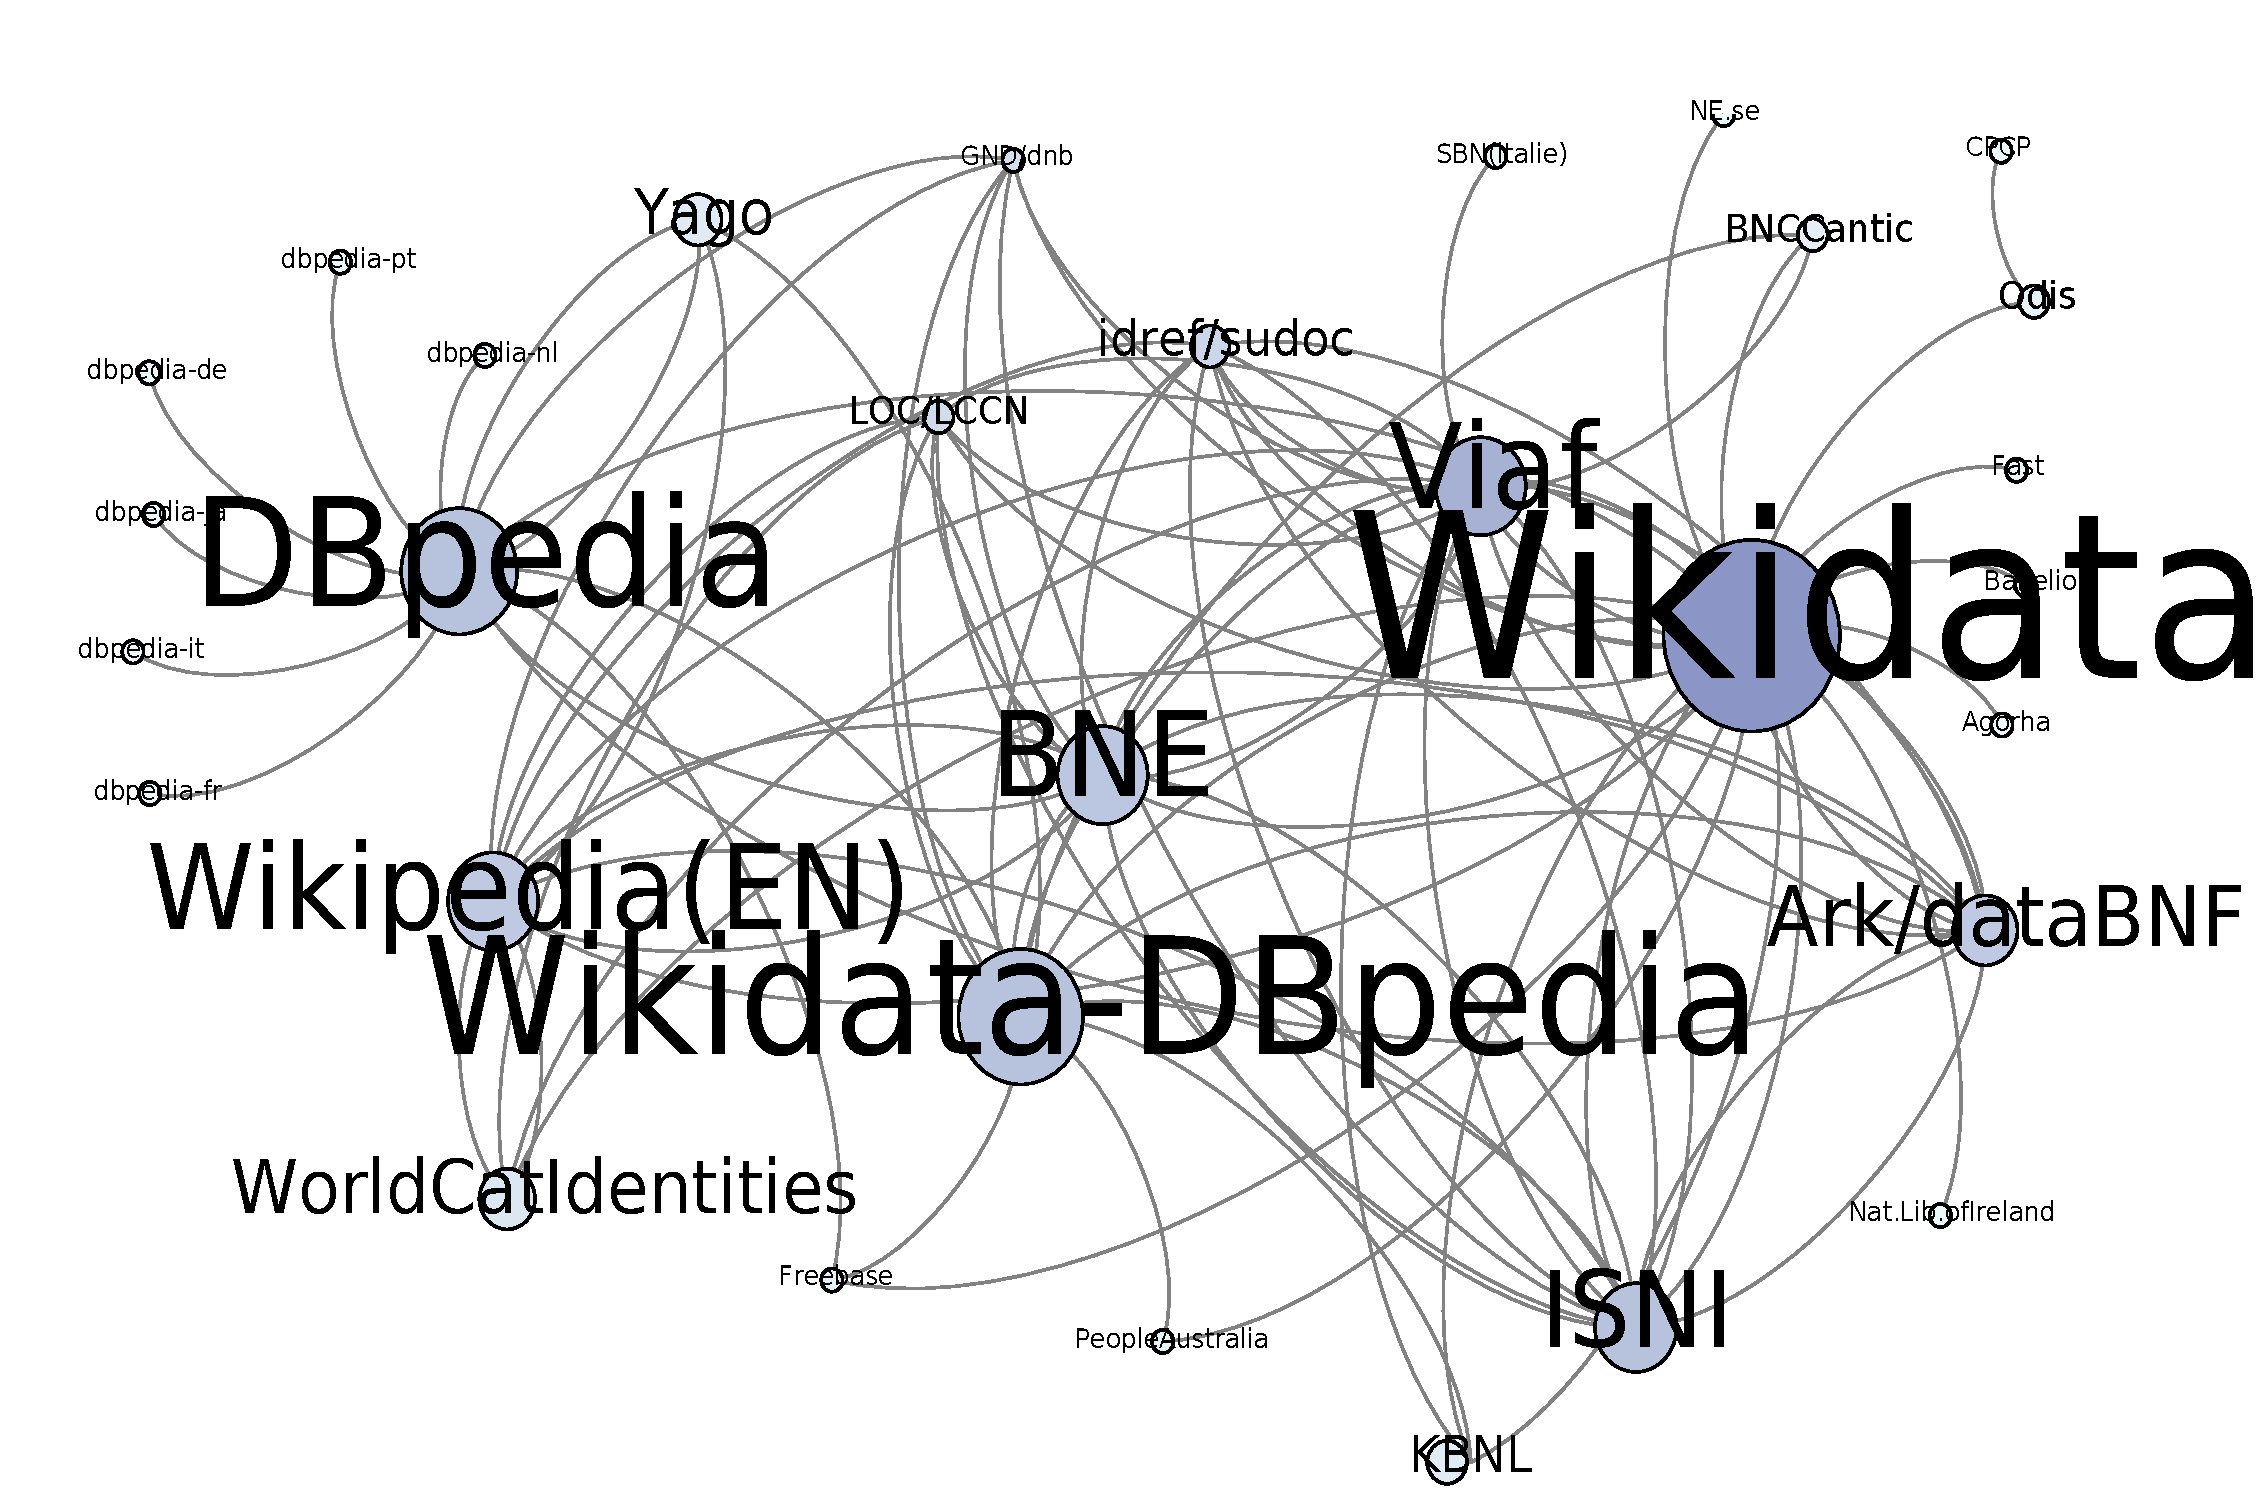
\includegraphics[scale=0.35]{../figures/figure1.pdf}

\caption{The part of the Linked Open Data graph traversed during the experiment.
The size of each node and label is proportional to the number of outgoing
links in the dataset.}

\end{figure}


\section{RDF Triples Harvesting}

During this process, ``Alex'' (i.e. : the authors) harvested more
than 22,000 RDF triples about Carton de Wiart. While this amount can
seem huge, it must be noted that the clear majority of these triples
are meaningless. RDF can be a very verbose format, requiring sometimes
a lot of triples to express something quite basic\footnote{Especially when institutions such as the Library of Congress provide
metadata about their triples, using RDF reification.}. Thus, once the useless triples eliminated, there are about 1,500
triples left, which use some 240 distinct properties.

However, these properties are often redundant, as each database uses
their own schemas. To encode a person's date of birth, for example,
YAGO uses the property \textsf{<\href{http://YAGO-knowledge.org/resource/infobox/en/birthdate}{http://YAGO-knowledge.org/resource/infobox/en/birthdate}>},
while DBpedia uses \textsf{<\href{http://dbpedia.org/ontology/birthDate}{http://dbpedia.org/ontology/birthDate}>}.
In order to facilitate the analysis, we have roughly classified the
various properties into eleven empirical classes: affiliations, appellations,
category, dates, descriptions, identifiers, locations, professions,
relations, works and miscellaneous. Figure~2 shows the proportion
of triples in each of these classes.

\begin{figure}
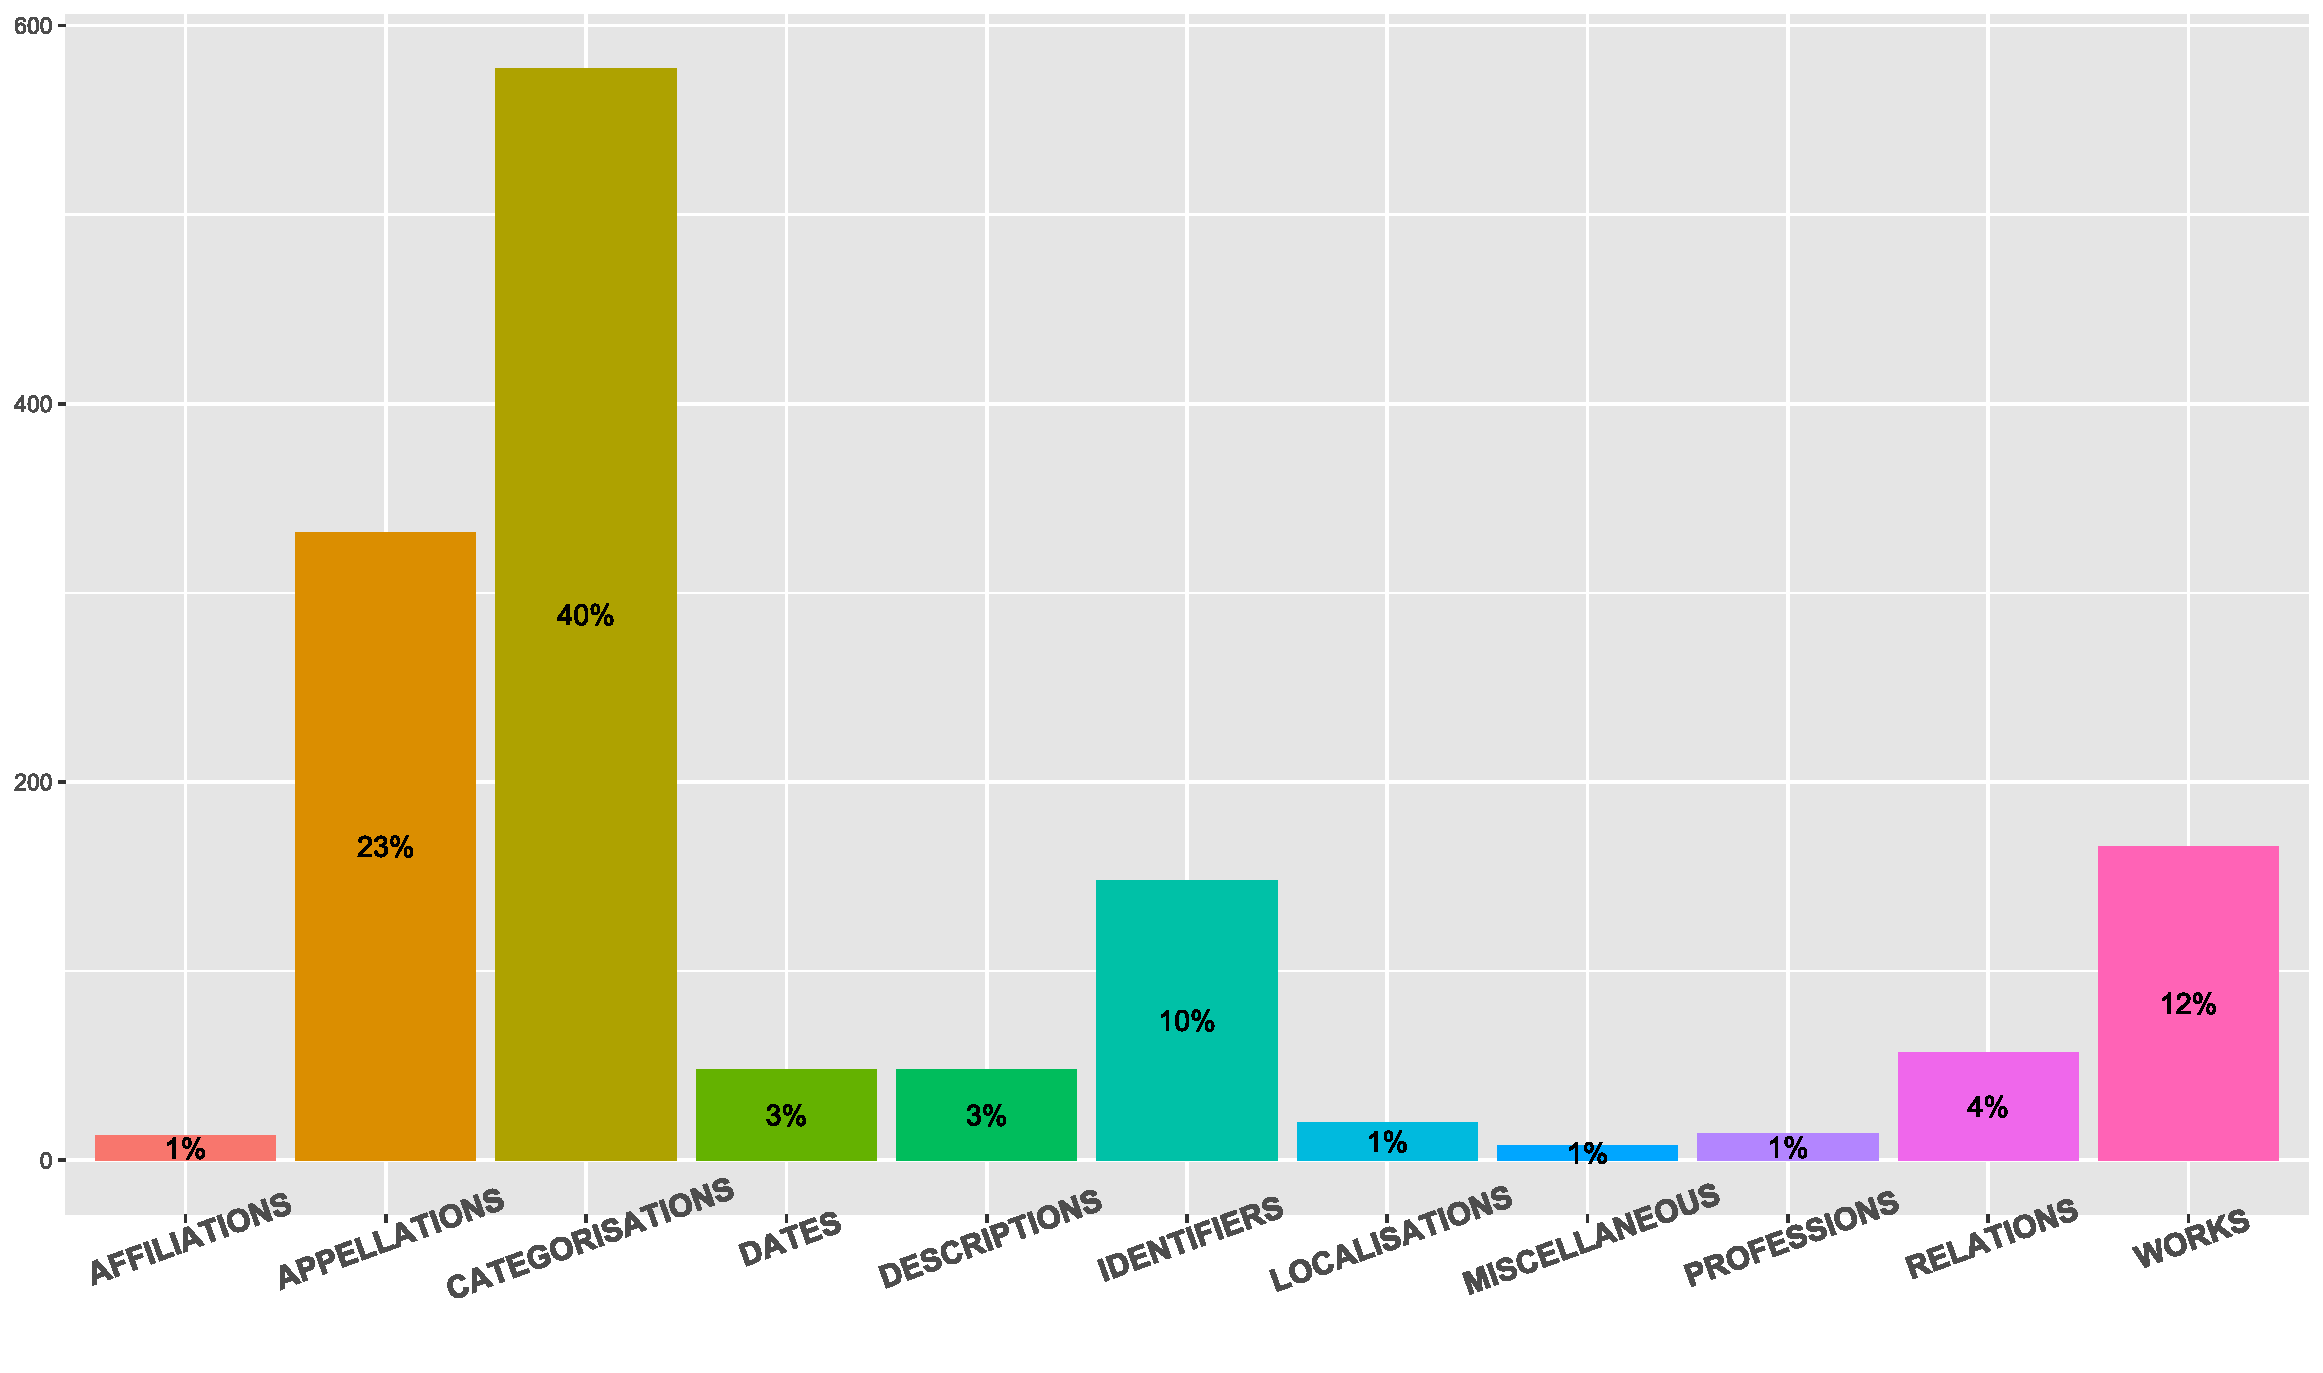
\includegraphics[scale=0.35]{../figures/figure2.pdf}

\caption{Distribution of properties manually divided into eleven classes.}

\end{figure}

Triples have been placed in their respective category according to
the property used. For instance, the property \textsf{<\href{http://www.w3.org/2000/01/rdf-schema\%5C\#label}{http://www.w3.org/2000/01/rdf-schema\textbackslash{}\#label}>}
corresponds to the ``appellation'' category, which encompasses all
the different labels used to refer to Henry Carton de Wiart. There
are many, especially in VIAF, which records the different labels used
by libraries: Carton de Wiart‏, Henry‏; Carton de Wiart, Henry,‏ Comte,
1869-1951‏; Carton de Wiart, Henry‏‎ (1869-1951)... The ``category''
class is the largest because it includes the (numerous) Wikipedia
and YAGO categories —for example \textsf{<\href{http://YAGO-knowledge.org/resource/wikicat_Walloon_people}{http://YAGO-knowledge.org/resource/wikicat\_Walloon\_people}>
or <\href{http://dbpedia.org/resource/Category:Members_of_the_Brussels_Guild_of_Saint_Luke}{http://dbpedia.org/resource/Category:Members\_of\_the\_Brussels\_Guild\_of\_Saint\_Luke}>}.

\section{Semi-Automated Biography}

Inspired by the aforementioned reports produced by robot journalists,
we tried to see what a biography based on RDF triples would look like.
To create this biography, we have synthesized the information contained
in the RDF triples collected by Alex. For the sake of clarity, we
present in Figure~3 a simplified version, based only on Wikidata
and three different versions of DBpedia (EN, FR, NL). This means that
this experimental biography does not contain the list of books that
Carton de Wiart wrote or collaborated on.

\begin{figure}

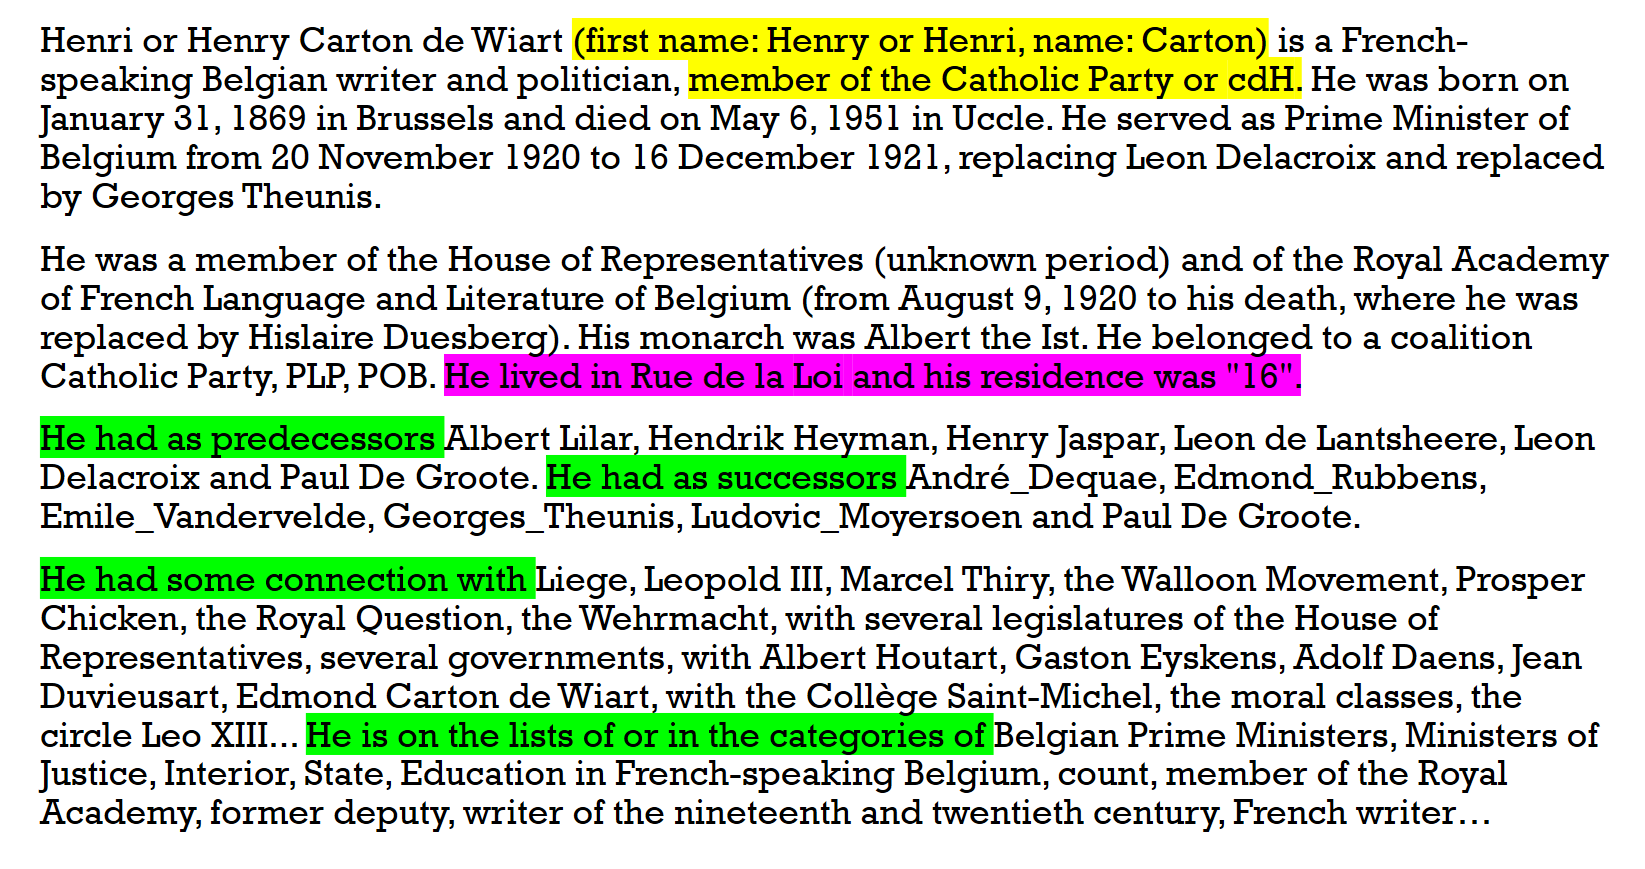
\includegraphics[scale=0.3]{../figures/figure3.png}\caption{Here is what an ``automated'' portrait of Henry Carton de Wiart
might look like based on information from the LOD Cloud.}
\end{figure}

As shown in Figure~3, all the text fits in less than 20 lines. The
result is far from Carton de Wiart's biography from the State Archives
of Belgium, let alone the 8-pages biographical note in the National
Biography. This confirms our first hypothesis: the overwhelming quantity
of triples are often redundant or useless. Most of them express the
same elements and often only offer basic information such as birth
and death dates. We have highlighted the most problematic excerpts.
The text in yellow points up contradictions. Firstly, it is not easy
to know how to write Henry. The spelling changes according to the
language. In Wikidata, the ``given name'' property is ``Henry'',
whereas DBpedia uses ``Henri''. Secondly, the Dutch version of DBpedia\footnote{\href{http://nl.dbpedia.org/page/Henri_Carton_de_Wiart}{http://nl.dbpedia.org/page/Henri\_Carton\_de\_Wiart}
(accessed 14 September 2018).} wrongly asserts that Carton de Wiart was a member of the ``cdH''
—a political party created in 2002, after his death. But other knowledge
bases correctly indicate that Wiart belonged to the Catholic party.

Moreover, the information is not always as structured and clear as
we could expect. For example, much of the information in DBpedia or
YAGO is not fully explicit. The Dutch version of DBpedia mentions
that Carton de Wiart belongs to the Wikipedia's ``List of Belgian
ministers of Justice''. However, this piece of information would
not be fully exploitable by a machine, not to mention the fact that
the years of his tenure as Minister of Justice are not even indicated.
Furthermore, the properties used by YAGO or DBpedia are often poorly
described or not described at all. It is therefore difficult to ascertain
what the ``successor'' property (highlighted in green in Figure~3)
covers. Successor of whom? For which function?

Similarly, it is doubtful that Carton de Wiart spent his entire life
at ``16 rue de la Loi'', official residence of the Belgian Prime
Ministers, presented in DBpedia as his home.

Finally, it appears that this text lacks essential biographical information,
for example about his studies or his family. Did he have a wife, children,
cousins, parents, siblings? This brings us to the next question: among
this missing information, which ones could be easily added and which
ones would be more difficult or impossible to translate into RDF?

\section{Manual ``Triplification''}

After this first exploration with the help of Alex-the-robot, we wanted
to take a close look at the data contained in less structured resources.
We tried to do that by acting as if we were an archivist wishing to
inject unstructured biographical information into the Linked Data
cloud. In other words, what the options would be to ``manually''
triplify extra information.

Different types of resources have been used: a biographical note from
the \emph{Biographie nationale de Belgique}, an EAC-CPF and an EAD
files from the State Archives. During this triplification process,
we considered each sentence, one after the other, and tried to extract
and translate every single piece of information about Carton de Wiart
into RDF triples (subject, predicate, object). For example, a single
sentence like ``Issu d'une famille de la noblesse catholique, Henry
Carton de Wiart effectua ses humanités au collège d'Alost puis au
collège Saint-Michel à Bruxelles, avant d'entreprendre des études
à l'Université libre de Bruxelles, où il obtint en 1890 son doctorat
en droit'' need at least seven different triples.

The whole triplification resulted in about 300 statements, containing
far more complete and detailed information than the Linked Data triples.
During this process, we observed several aspects which can lead to
the loss of information, which in turn makes it difficult to deliver
a clear and representative description of Henry Carton de Wiart. We
have identified three types of challenges, which are respectively
related to the data, to the triple structure and to the vocabulary. 
\begin{itemize}
\item Albeit the completeness of the data available can constitute a limit,
a more challenging point is the granularity: besides practical aspects
and available human resources, at what level of detail should a personality
and his life be described? For example, in an archival context, should
we only use the biographical section of the EAD or also take into
consideration other levels of description? 
\item The triple structure of RDF requires a different way of expressing
things. For instance, the translation of one single sentence results
sometimes in five or six different triples because of the reification
principle.
\item If a piece of knowledge can be expressed by words in a biography,
like ``Henry had four brothers'', its full description sometimes
has to be inferred from other statements in the RDF language (for
example counting the number of triples that use a property like \textsf{brotherOf}).
\item Several RDF vocabularies can be used to specify the relationship between
persons. Again, we noticed some limits related to granularity. Thus,
in the family context, depending on what vocabulary we used, we were
able to specify that someone was an uncle, or merely describe the
fact that he was a relative. In this case, we would lose details and
have uncle and cousin described by the same vague property. 
\item For social relationship, the vocabulary BIO\footnote{\href{https://lov.linkeddata.es/dataset/lov/vocabs/bio}{https://lov.linkeddata.es/dataset/lov/vocabs/bio}
(accessed 14 September 2018).} allows to qualify ``acquaintance of'', ``friend of'', ``a close
friend of'', ``has met'', etc. Although this representation is
useful, sometimes it seems quite difficult to evaluate the specific
nature of a relationship between two dead people... 
\item During the triplification process, most of the data has been translated
in RDF triples without issues. In a few cases, we lacked vocabulary
terms to express more atypical statements, such as details about Henry's
personality, or mentions about his activism in the context of social
struggles. Obviously, it raises the question of the long tail : to
what extent should we create new properties for each very specific
case?
\end{itemize}

\section{Conclusion and Next Steps}

We have seen in this experiment that the Linked Open Data cloud contains
a lot of triples about Carton de Wiart, but the total amount of information
is quite poor. We have also seen that many other biographical elements
can be added as RDF triples, and that there is often a controlled
vocabulary that can express them.

But creating our own RDF files requires time and skills. So, another
approach might be to automatically feed Wikidata, which can be edited
by users unlike DBpedia. In the coming months, we will explore these
tracks. We will also try to generalize this first small experiment
on a wider panel of personalities and entities, for example organizations
or historical events. In other words, we will leave the close reading
approach to return to a more classical distant reading.
\end{document}
